\documentclass[12pt,a4paper]{article}
\usepackage{cmap}
\usepackage[T2A]{fontenc}
\usepackage[utf8]{inputenc}
\usepackage[russian]{babel}
\usepackage{amsmath,amssymb,geometry,graphicx,float,hyperref,array,longtable}
\usepackage[labelfont=bf]{caption}
\geometry{left=20mm,right=20mm,top=20mm,bottom=20mm}
\captionsetup{skip=5pt}
\captionsetup[table]{justification=raggedright,singlelinecheck=false}
\addto\captionsrussian{\renewcommand{\figurename}{Рисунок}}
\hypersetup{hidelinks,pdftitle={Лабораторная работа 2. Принцип максимума. Вариант 11},
  pdfauthor={Иванов Никита Михайлович}}
\setlength{\emergencystretch}{2em}
\setlength{\intextsep}{8pt}
\graphicspath{{results/}}
\makeatletter
\def\tagform@#1{\maketag@@@{\ignorespaces#1\unskip\@@italiccorr}}
\makeatother

\title{Лабораторная работа №2\\
Синтез оптимального управления. Принцип максимума\\
Вариант 11}
\author{Иванов Никита Михайлович\\Группа R3436}
\date{10 ноября 2026 г.}

\begin{document}
\maketitle
\newpage
\tableofcontents
\newpage

\section{Постановка задачи}
Требуется построить оптимальный регулятор, промоделировать его работу
и исследовать изменение критерия при отклонении параметров регулятора.
Для варианта 11 уравнения объекта имеют вид
\begin{equation}
  \dot{x}_1=4x_2,\qquad \dot{x}_2=x_1+u .
\end{equation}
Время перехода задано: $T=9$~с. Оба конца траектории закреплены:
\[
  x(0)=\begin{pmatrix}0\\0\end{pmatrix},\qquad
  x(T)=\begin{pmatrix}1\\0\end{pmatrix}.
\]
Необходимо минимизировать интегральный критерий
\begin{equation}
  J[u]=\int_0^T\bigl(x_1^2+2x_1x_2+9x_2^2+7u^2\bigr)\,dt .
\end{equation}
Ограничения на амплитуду $u$ отсутствуют. В матричной форме
$\dot x=Ax+Bu$, а подынтегральная функция равна $x^{\mathsf T}Qx+7u^2$, где
\[
  A=\begin{pmatrix}0&4\\1&0\end{pmatrix},\qquad
  B=\begin{pmatrix}0\\1\end{pmatrix},\qquad
  Q=\begin{pmatrix}1&1\\1&9\end{pmatrix}.
\]

\section{Принцип максимума Понтрягина}
Введём сопряжённые переменные $p=(p_1,p_2)^{\mathsf T}$.
Для минимизации $J$ возьмём гамильтониан
\begin{equation}
  H=4p_1x_2+p_2(x_1+u)-x_1^2-2x_1x_2-9x_2^2-7u^2 .
\end{equation}
Условие $\partial H/\partial u=p_2-14u=0$ определяет
управление $u^*=p_2/14$. Вторая производная по $u$ равна $-14$,
поэтому это единственная точка максимума $H$ по $u$ при заданных $x$ и $p$.
Сопряжённые уравнения имеют вид
\begin{equation}
  \dot p_1=-p_2+2x_1+2x_2,\qquad
  \dot p_2=-4p_1+2x_1+18x_2 .
\end{equation}
Вместе с уравнениями объекта и законом $u^*=p_2/14$ они образуют
краевую задачу. Четыре краевых условия заданы для координат $x_1,x_2$
в моменты $0$ и $T$. Значения сопряжённых переменных определяются из решения.

\clearpage
\section{Оптимальная траектория}
\subsection{Решение краевой задачи}
Обозначим $q=x_1^*$. Из уравнений объекта и условия максимума следуют
\[
  x_2^*=\frac{q'}{4},\qquad
  u^*=\frac{q''}{4}-q,\qquad
  p_2=\frac{7}{2}q''-14q,\qquad
  p_1=\frac12 q+\frac{37}{8}q'-\frac78q''' .
\]
Подставляя $p_1$ и $p_2$ в первое сопряжённое уравнение, получаем
\begin{equation}
  7q^{(4)}-65q''+128q=0,\qquad
  q(0)=q'(0)=0,\quad q(T)=1,\quad q'(T)=0.
\end{equation}
Характеристические корни равны $\pm r_1,\pm r_2$, где
\[
  r_1=\sqrt{\frac{65-\sqrt{641}}{14}}\approx1.683577,\qquad
  r_2=\sqrt{\frac{65+\sqrt{641}}{14}}\approx2.539938 .
\]
Запишем решение в экспонентах, убывающих от концов интервала:
\begin{equation}
  q(t)=a_1 e^{-r_1 t}+a_2 e^{-r_2 t}
       +b_1 e^{-r_1(T-t)}+b_2 e^{-r_2(T-t)}.
  \label{eq:profile}
\end{equation}
Для строки $f(t)=(e^{-r_1t},e^{-r_2t},e^{-r_1(T-t)},e^{-r_2(T-t)})$
система для столбца коэффициентов имеет вид
\[
  \begin{pmatrix} f(0)\\ f'(0)\\ f(T)\\ f'(T)\end{pmatrix}
  \begin{pmatrix}a_1\\a_2\\b_1\\b_2\end{pmatrix}
  =\begin{pmatrix}0\\0\\1\\0\end{pmatrix}.
\]
Отсюда $a_1\approx-3.841627\cdot10^{-6}$, $a_2\approx3.062650\cdot10^{-6}$,
$b_1\approx2.965965$, $b_2\approx-1.965965$.

\subsection{Обоснование глобального минимума}
Пусть $y=x-x^*$ и $v=u-u^*$ задают отклонение допустимой траектории.
Тогда $\dot y=Ay+Bv$ и $y(0)=y(T)=0$. Из
$\dot p=2Qx^*-A^{\mathsf T}p$ и $B^{\mathsf T}p=14u^*$ следует
\[
  \frac{d}{dt}(p^{\mathsf T}y)=2(x^*)^{\mathsf T}Qy+14u^*v .
\]
При разложении $J[u]-J[u^*]$ интеграл от линейных по $y,v$ членов
равен $[p^{\mathsf T}y]_0^T=0$. Поэтому
\begin{equation}
  J[u]-J[u^*]=\int_0^T\bigl(y^{\mathsf T}Qy+7v^2\bigr)\,dt\geq0 .
  \label{eq:costdifference}
\end{equation}
Здесь $y^{\mathsf T}Qy=(y_1+y_2)^2+8y_2^2$.
Равенство возможно только при совпадении траекторий и совпадении
управлений почти всюду. Следовательно, найденное управление
обеспечивает единственный глобальный минимум.

\clearpage
\section{Регулятор и моделирование}
Оптимальные сигналы $x^*(t)$ и $u^*(t)$, полученные из
формулы~\eqref{eq:profile}, задают программу движения. Для её отслеживания
используем закон управления
\begin{equation}
  u(t,x)=u^*(t)-K\bigl(x-x^*(t)\bigr),\qquad
  K=\begin{pmatrix}5/2&5\end{pmatrix}.
\end{equation}
Ошибка отслеживания $e=x-x^*$ подчиняется уравнению
$\dot e=(A-BK)e$. Коэффициенты $K$ выбраны так, чтобы собственные
числа $A-BK$ были равны $-2$ и $-3$. При заданном начальном
состоянии $e(0)=0$, поэтому регулятор реализует оптимальное движение.

При моделировании вместе с уравнениями объекта интегрировалось
уравнение накопленного критерия
\[
  \dot J(t)=x^{\mathsf T}Qx+7u^2,\qquad J(0)=0.
\]
Результаты приведены на рисунке~\ref{fig:signals}. В момент $T=9$~с
выполнены условия $x_1(T)=1$, $x_2(T)=0$ и получено
$J(T)=8.151471957$. Это значение также следует из равенства
$\frac{d}{dt}(p^{\mathsf T}x^*)=2(x^*)^{\mathsf T}Qx^*+14(u^*)^2$,
которое даёт $J[u^*]=p_1(T)/2$.

\begin{figure}[H]
  \centering
  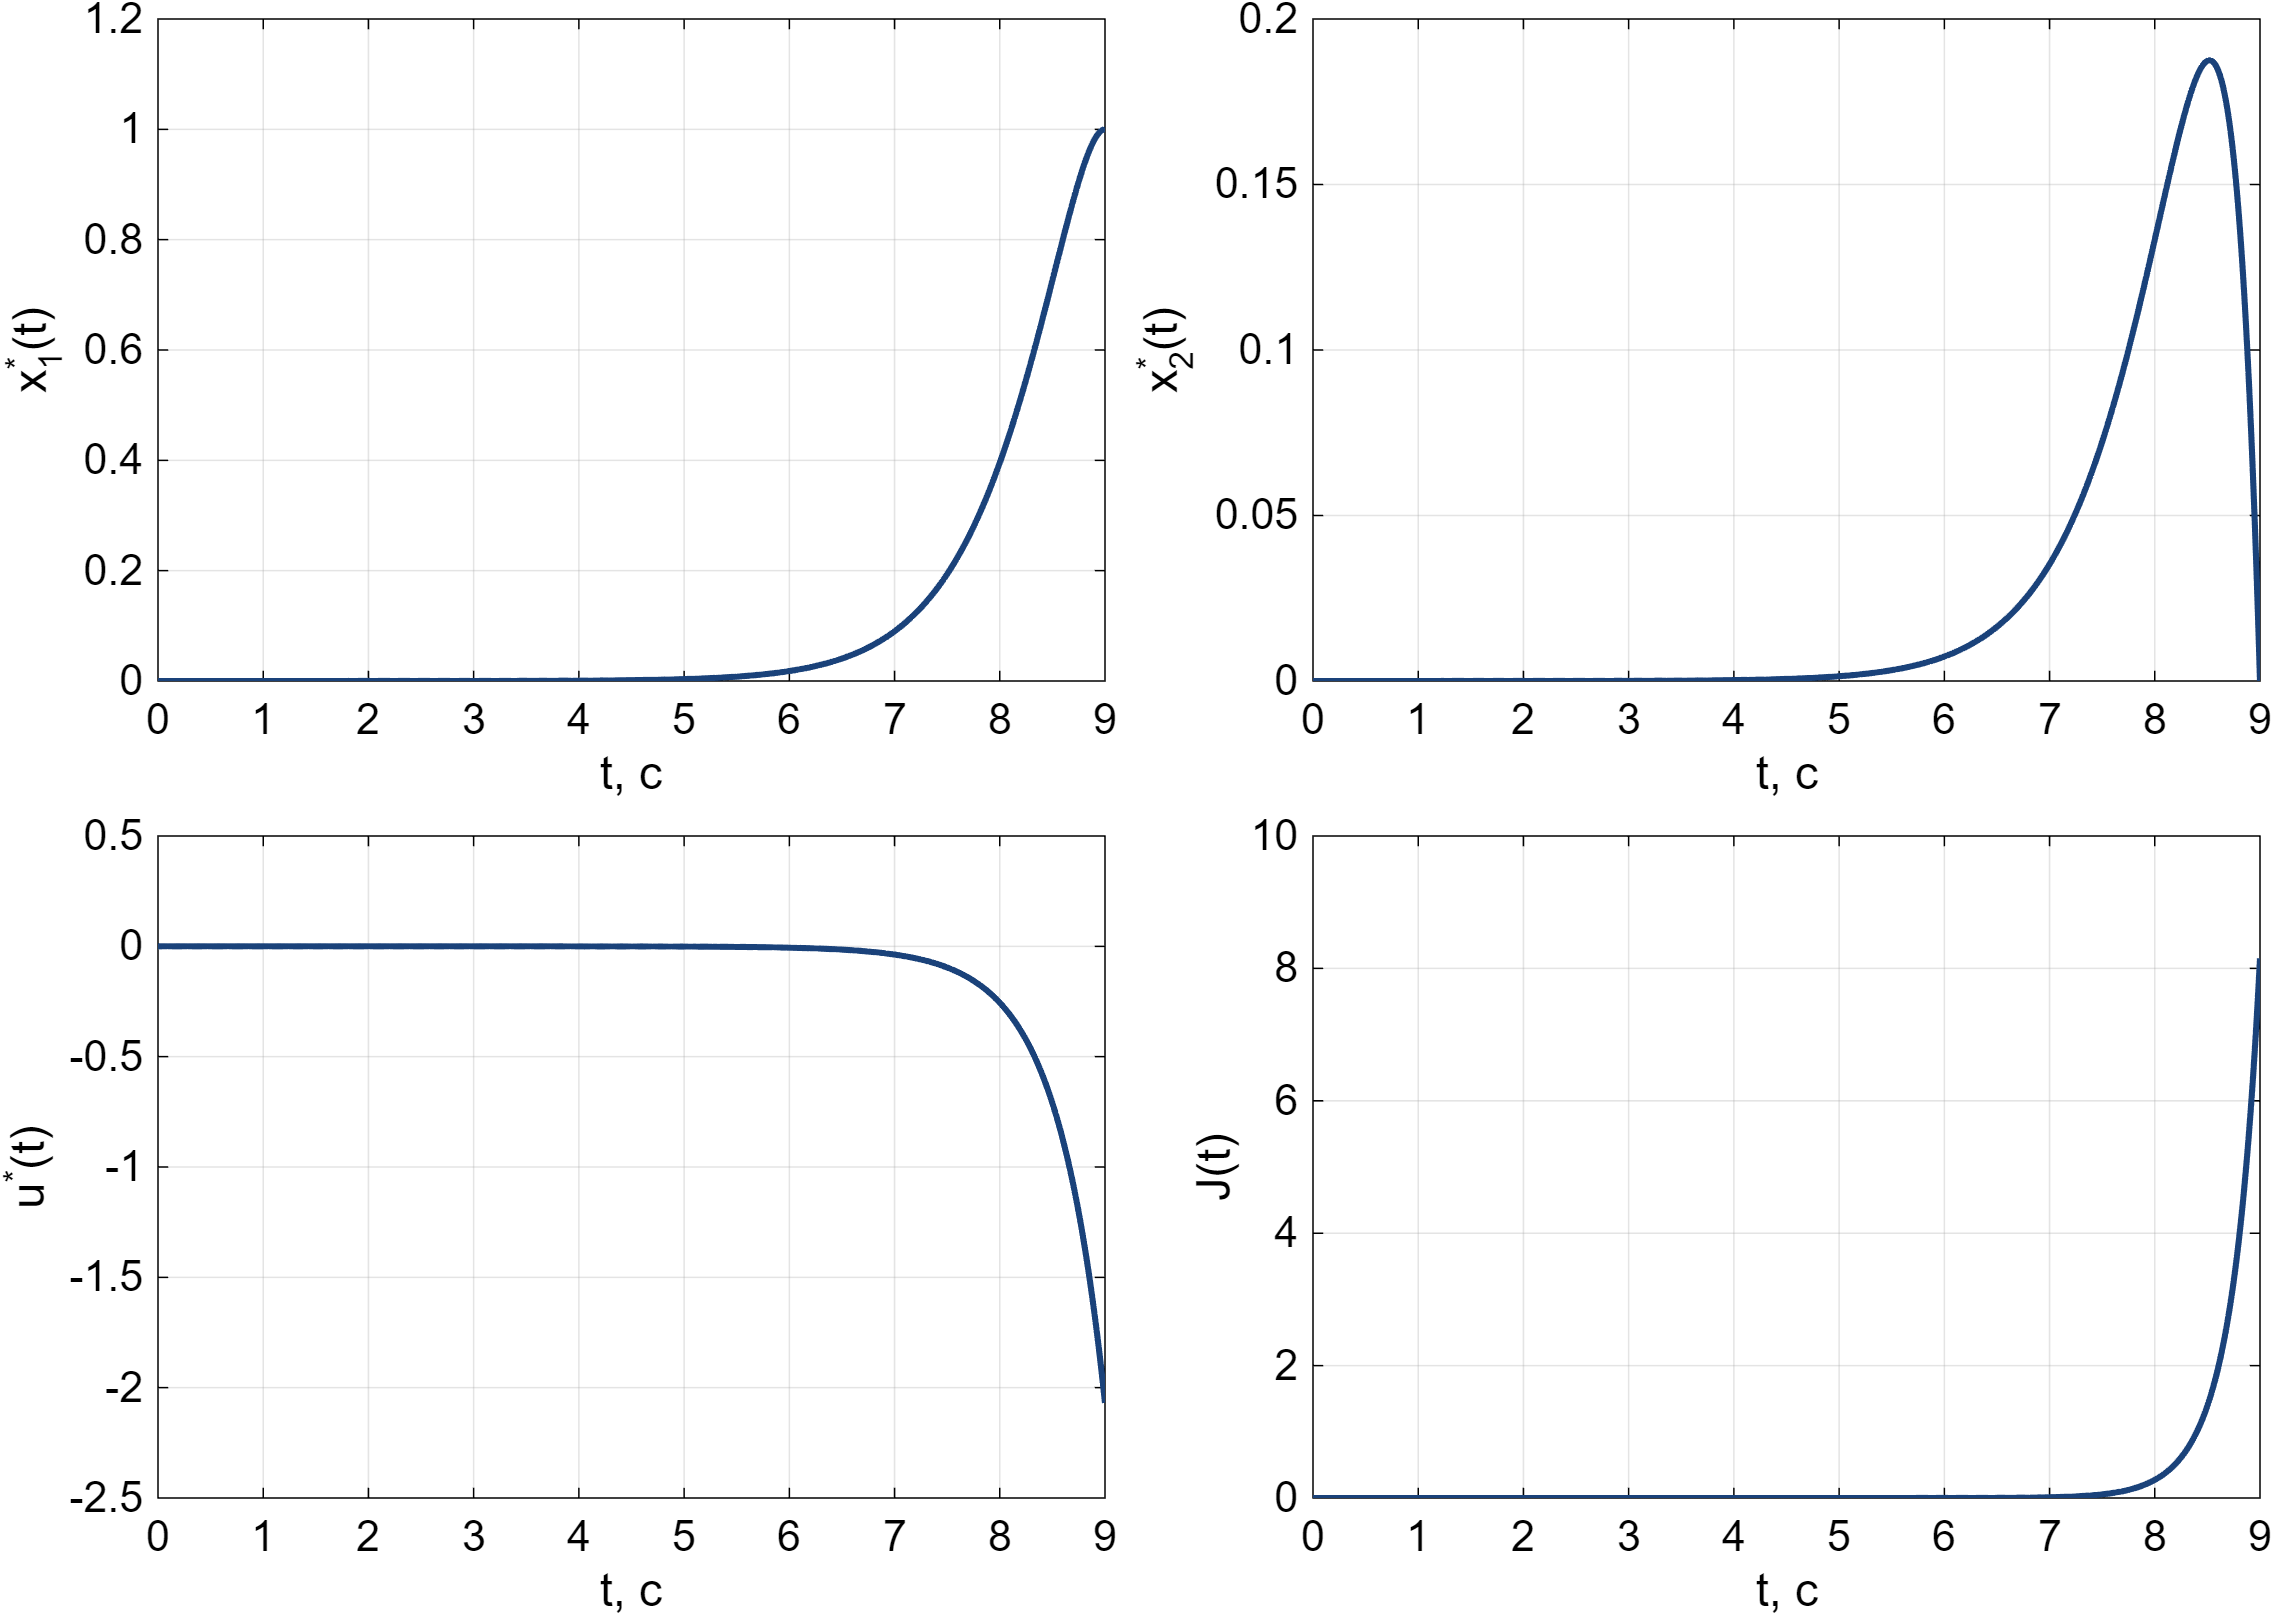
\includegraphics[width=\textwidth]{optimal_signals.png}
  \caption{Оптимальные траектории, управление и накопленный критерий}
  \label{fig:signals}
\end{figure}

За первые восемь секунд накопленный критерий достигает $J(8)\approx0.273645$.
Около $96.6\%$ полного значения критерия набирается за последнюю секунду.

\clearpage
\section{Отклонение параметров регулятора}
Сохраним коэффициенты обратной связи и введём два параметра программы.
Коэффициент $k$ масштабирует оптимальную траекторию, а $\alpha$ меняет
её форму. При $s=t/T$ зададим $h(t)=16s^2(1-s)^2$ и положим
\[
  x_{\mathrm{ref}}=k x^*+\alpha
  \begin{pmatrix}h\\h'/4\end{pmatrix},\qquad
  u_{\mathrm{ref}}=k u^*+\alpha(h''/4-h).
\]
Регулятор использует $u=u_{\mathrm{ref}}-K(x-x_{\mathrm{ref}})$.
Оптимальной программе соответствуют $k=1$, $\alpha=0$.
Поскольку $h=h'=0$ на обоих концах интервала, конечное состояние
равно $(k,0)^{\mathsf T}$ при любом $\alpha$.

\subsection{Изменение масштаба}
При $\alpha=0$ значение критерия равно $k^2J[u^*]$.
В таблице~\ref{tab:scale} приведены результаты при изменении $k$ на
$\pm5\%$ и $\pm10\%$. При $k<1$ критерий уменьшается, но целевая
координата $x_1(T)=1$ не достигается.

\begin{table}[H]
  \centering
  \caption{Результаты при изменении масштаба программы}
  \label{tab:scale}
  \begin{tabular}{|c|c|c|r|}
    \hline
    $k$ & $x_1(T)$ & $J(T)$ & Изменение $J$, \% \\ \hline
    $0.90$ & $0.90$ & $6.602692$ & $-19.00$ \\
    $0.95$ & $0.95$ & $7.356703$ & $-9.75$ \\
    $1.00$ & $1.00$ & $8.151472$ & $0.00$ \\
    $1.05$ & $1.05$ & $8.986998$ & $+10.25$ \\
    $1.10$ & $1.10$ & $9.863281$ & $+21.00$ \\ \hline
  \end{tabular}
\end{table}

\subsection{Изменение формы при фиксированном конце}
При $k=1$ все переходы удовлетворяют обоим краевым условиям.
Максимум $h$ равен единице, поэтому $\lvert\alpha\rvert$ задаёт
максимальное отклонение $x_1(t)$ от оптимальной траектории.
Из равенства~\eqref{eq:costdifference} и интегрирования по частям следует
\[
  J(1,\alpha)=J[u^*]+\alpha^2 C,\qquad
  C=\int_0^T\left(8h^2+\frac{65}{16}(h')^2+\frac{7}{16}(h'')^2\right)dt
    \approx31.581109 .
\]

\begin{table}[H]
  \centering
  \caption{Результаты при изменении формы программы}
  \label{tab:shape}
  \begin{tabular}{|c|c|r|}
    \hline
    $\alpha$ & $J(T)$ & Изменение $J$, \% \\ \hline
    $0$ & $8.151472$ & $0.00$ \\
    $\pm0.05$ & $8.230425$ & $+0.97$ \\
    $\pm0.10$ & $8.467283$ & $+3.87$ \\ \hline
  \end{tabular}
\end{table}

\section{Выводы}
По принципу максимума Понтрягина построено управление, которое за
$9$~с переводит систему из $(0,0)$ в $(1,0)$ и обеспечивает
глобальный минимум $J^*\approx8.151472$. Моделирование подтвердило
достижение конечного состояния и расчётное значение критерия.
При изменении формы программы с сохранением конечного состояния
критерий возрастает пропорционально квадрату отклонения
(таблица~\ref{tab:shape}). Изменение масштаба программы приводит к промаху
по конечной координате (таблица~\ref{tab:scale}).
\end{document}
